%%%
%%%  ___ _                     __  __ _           _
%%% | _ |_)__ _ _ _  __ __ _  |  \/  (_)_  _ __ _| |__  ___
%%% | _ \ / _` | ' \/ _/ _` | | |\/| | | || / _` | '_ \/ -_)
%%% |___/_\__,_|_||_\__\__,_| |_|  |_|_|\_, \__,_|_.__/\___|
%%%                                     |__/
%%%
%%% PROJETO DE TCC: Documento modelo em LaTeX, padrão ABNT usando ABNTeX2
%%%
%%% ----------------------------------------------------------------------------
%%%
%%% Para compilar, na linha de comando:
%%%
%%%
%%%    latexmk -lualatex skeleton_tcc_proj.tex
%%%
%%% ----------------------------------------------------------------------------
%%%
%%% By Cantão! <rfcantao@gmail.com>
%%% Baseado em template do Prof. James A. Souza
%%%

\documentclass[11pt,oneside,brazil,hidelinks,article,sumario=tradicional,a4paper]{abntex2}

% Pacotes padrão da American Mathematical Society
\usepackage{amsmath}
\usepackage{amssymb}
\usepackage{mathtools}
\usepackage{indentfirst}


%%%
%%% São usadas as fontes:
%%% - Crimsom Pro: texto principal
%%% - Noto Sans: sem serifa, usada nas seções, subseções, etc
%%% - DejaVu Sans Mono: monoespaçada para listagems, URLs, etc
%%%
\usepackage{fontspec}
% CrimsonText é similar à Minion Pro, que é comercial
\setmainfont{CrimsonPro}[
  Path           = ./fonts/,
  Extension      = .ttf,
  UprightFont    = *-Regular,
  BoldFont       = *-Bold,
  ItalicFont     = *-Italic,
  BoldItalicFont = *-BoldItalic,
  SmallCapsFont  = AlegreyaSC-Regular
]
% NotoSans é similar à Myriad Pro, que é comercial
\setsansfont{NotoSans}[
  Path           = ./fonts/,
  Extension      = .ttf,
  UprightFont    = *-Regular,
  BoldFont       = *-Bold,
  ItalicFont     = *-Italic,
  BoldItalicFont = *-BoldItalic
]
\setmonofont{DejaVuSansMono}[
  Path           = ./fonts/,
  Extension      = .ttf,
  UprightFont    = *,
  BoldFont       = *-Bold,
  ItalicFont     = *-Oblique,
  BoldItalicFont = *-BoldOblique,
  Scale          = MatchLowercase
]

\usepackage[math-style=TeX]{unicode-math}
%\setmathfont{Asana-Math.otf}[Scale=MatchLowercase]
\setmathfont{STIXTwoMath-Regular.otf}[Scale=MatchLowercase]
%\setmathfont{texgyredejavu-math.otf}[Scale=MatchLowercase]


%%%
%%% Idiomas: Português e Inglês
%%%
%%% Certifique-se de ter os pacotes corretos (GNU/Linux):
%%%   sudo apt install texlive-lang-en texlive-lang-portuguese texlive-xetex
%%%
%%% O TeXLive (recomendo no caso do Windows) em geral já tem esses pacotes instalados
%%%
\usepackage{polyglossia}
\setmainlanguage{portuges}
\setotherlanguage{english}
\usepackage{csquotes}

%%%
%%% Outros pacotes úteis
%%%
\usepackage{graphicx}  % Figuras em vários formatos (png, pdf)
\usepackage{color}     % Cores
\usepackage{pgfgantt}  % Cronogramas
\usepackage{multicol}  % Documentos com várias colunas
\usepackage{booktabs}  % Tabelas profissionais
\usepackage[final]{microtype}
\usepackage{siunitx}   % Pacote para unidades físicas (recomendo muito!)
\sisetup{output-decimal-marker={,}}
\sisetup{mode=text}
\usepackage{braket}
\usepackage{makecell}

%%%
%%% CORES MANEIRÍSSIMAS
%%%
\definecolor{green}{RGB}{174,226,57}    % colourlovers.com/palette/46688/fresh_cut_day (atomic bikini)
\definecolor{yellow}{RGB}{237,229,116}  % colourlovers.com/palette/937624/Dance_To_Forget (Give Your Heart)
\definecolor{orange}{RGB}{255,164,70}   % colourlovers.com/palette/1107950/Indecent_Proposal (exotic orange)
\definecolor{onlyorange}{RGB}{191,77,40}% colourlovers.com/palette/953498/Headache (Only Orange)
\definecolor{cyan}{RGB}{108,243,213}    % colourlovers.com/palette/940927/Acused (wrong cyan)
\definecolor{red}{RGB}{199,8,8}         % colourlovers.com/palette/79468/LipstickOnHisCollar (Flagged Down)
\definecolor{melon}{RGB}{209,49,92}     % colourlovers.com/palette/2350697/This_is_for_YOU! (melon)
\definecolor{blue}{RGB}{62,122,162}     % colourlovers.com/palette/794774/be_here_for_me (kreuger)
\definecolor{berry}{RGB}{95,13,59}      % colourlovers.com/palette/117122/BurberryTenderTouch (BurberryTender)
\definecolor{violet}{RGB}{87,30,240}    % From the original template (Violet Thanos)
\definecolor{hymnroyale}{RGB}{42,4,72}  % colourlovers.com/palette/81885/Hymn_For_My_Soul (Hymn Royale)
\definecolor{think}{HTML}{607848}       % colourlovers.com/palette/38562/Hands_On
\definecolor{gray}{HTML}{444444}
\definecolor{intelligentsia}{RGB}{7,69,111} % colourlovers.com/palette/4792400/Intelligentsia (Intelligentsia circle)

\usepackage{tcolorbox}
\tcbuselibrary{many}
\tcbuselibrary{theorems}

\newtcbtheorem[number within=section]{theo}{Teorema}{
  enhanced,
  %skin=bicolor,
  arc=0mm,
  colback=black!3,
  colframe=black!50,
  colbacktitle=white,
  colbacklower=white,
  coltitle=black,
  fonttitle=\small,
  toptitle=3pt,
  bottomtitle=3pt,
  top=5pt,
  bottom=5pt,
  left=10pt,
  right=10pt,
  boxrule=0pt,
  titlerule=0pt}{th}

%%%
%%% Informações do PDF
%%%
\makeatletter
\hypersetup{%
  pdftitle={\@title},
  pdfauthor={\@author},
  pdfsubject={\imprimirpreambulo},
  pdfcreator={LuaLaTeX with abnTeX2},
  pdfkeywords={tcc}{licenciatura em física}{projeto de pesquisa},
  colorlinks=true,    % false: boxed links; true: colored links
  linkcolor=gray,     % color of internal links
  citecolor=gray,     % color of links to bibliography
  filecolor=gray,     % color of file links
  urlcolor=gray,
  bookmarksdepth=4
}
\makeatother

%%%
%%% Bibliografia
%%%
%%% Aqui estamos usando por padrão um programa chamado 'biber'. Ele é o responsável
%%% por converter o arquivo 'skeleton.bib' nas referências formatadas no padrão
%%% ABNT.
%%%
%%% Para saber mais:
%%% https://www.overleaf.com/learn/latex/Bibliography_management_in_LaTeX
%%%
\usepackage[backend=biber,style=abnt,noslsn,repeatfields]{biblatex}
\addbibresource{./tcc.bib}

%%% Função seno em PT-BR
\DeclareMathOperator{\sen}{sen}

%%%
%%% Configurações do documento para ABNTeX2
%%%
\titulo{Simulação de Circuitos Quânticos para o estudo de ruídos no fenômeno de teletransporte quântico}
\autor{Bianca Miyabe Santos Freitas}
\orientador{Prof. Dr. Renato Fernandes Cantão}
\instituicao{%
  UNIVERSIDADE FEDERAL DE SÃO CARLOS --- \textsl{CAMPUS} SOROCABA
  \par
  CENTRO DE CIÊNCIAS E TECNOLOGIAS PARA A SUSTENTABILIDADE
  \par
  DEPARTAMENTO DE FÍSICA, QUÍMICA E MATEMÁTICA}
\tipotrabalho{Projeto de Trabalho de Conclusão de Curso}
\preambulo{Projeto de Trabalho de Conclusão de curso apresentado ao curso de Licenciatura Plena em Física da Universidade Federal de São Carlos, \textsl{Campus} Sorocaba, como requisito para a conclusão da disciplina TCC 1.}
\local{Sorocaba}
\data{Abril, 2022}

% Modelo sugerido pela UFSCar
\renewcommand{\imprimircapa}{%
  \begin{capa}%
    \centering
    {\imprimirinstituicao\vfill}

    {\ABNTEXchapterfont\large\imprimirautor}

    \vfill
    {\ABNTEXchapterfont\bfseries\LARGE\imprimirtitulo}
    \vfill

    \large\imprimirlocal

    \large\imprimirdata

    \vspace*{15mm}
  \end{capa}
}

\begin{document}

%%% Elementos pré-textuais (capa, sumário, etc)
\pretextual
\imprimircapa
% \imprimirfolhaderosto

\begin{resumo} % Resumo em PT-BR
%  O resumo é um mini projeto de pesquisa onde deve conter uma breve descrição de toda a proposta, desde a área de pesquisa, referencial teórico no caso de ensino, teoria, experimento, objetivos a serem alcançados, metodologia e resultados esperados. Este deve indicar quais questões vocês (aluno e orientador), como pesquisadores, pretendem responder, permitindo ao leitor acessar rapidamente a ideia básica e os objetivos de sua proposta. O resumo deve ser escrito em um único parágrafo sem espaçamento no início, como nesse exemplo.
  \vspace{\onelineskip}

  \noindent
%  \textbf{Palavras-chave}: são aquelas que mais aparecem no texto especificando o fenômeno em estudo, a área de concentração, alguma técnica específica, etc. Pelo menos três palavras e no máximo cinco, separadas por ponto (Palavra 1. Palavra 2. Palavra 3).
\end{resumo}
\newpage


\begin{resumo}[Abstract] % Resumo em EN
  \begin{otherlanguage*}{english}
 %   Same as above, but in English.
    \vspace{\onelineskip}

    \noindent
%    \textbf{Keywords}: Word 1. Word 2. Word 3.
  \end{otherlanguage*}
\end{resumo}
\newpage


%%% Caso já seja um trabalho final
% \listoffigures*
% \clearpage

% \listoftables*
% \clearpage

% \tableofcontents*
% \clearpage

%%% Pular página
% \clearpage

%%% Elementos textuais (o documento em si)
\textual%

%%%
%%% INTRODUÇÃO
%%%
\section{Introdução}\label{sec:intro}


Segundo \textcite{conceitoinformação}, o conceito de informação possui seu significado cotidianamente atribuído como \textit{conhecimento comunicado}. Nesse sentido, a informação já existia nas pinturas rupestres há cerca de \num{45,5} mil anos atrás, nas quais estão registradas uma série de imagens no intuito de comunicar, seja um evento ou ainda uma quantidade. Apesar do conceito de informação aparecer desde os primórdios do estabelecimento da humanidade, é apenas na década de 1940 que esta passa a ser objeto de estudo com os trabalhos de Claude Elwood Shannon (1916--2001), que desenvolve uma teoria matemática para a informação \cite{CiênciaTransiçãoSeculosa}.

O objetivo principal da Teoria da Comunicação de Shannon ou \textit{Teoria Matemática da Comunicação} (TMC), consistiu em sistematizar o conhecimento acumulado até então, acerca da eficiência em sistemas de comunicação. A teoria descreve o funcionamento lógico-matemático de um destes sistemas, composto por um gerador de informação, um meio de transmissão e um receptor, conforme ilustra a Figura~\ref{comunicshannon} \cite{MTC}.

\begin{figure}[ht!]
  \centering
  \caption{Esquema geral de um sistema de comunicação com a Fonte de Informação (\textit{Information Source}) criando uma Mensagem (\textit{Message}) a ser transmitida pelo Transmissor (\textit{Transmitter}) que a transforma em um Sinal (\textit{Signal}). Na transmissão pode haver uma Fonte de Ruído (\textit{Noise Source}). O sinal é recebido (\textit{Received Signal}) pelo Receptor (\textit{Receiver}) e finalmente a mensagem chega ao seu Destino (\textit{Destination}).}\label{comunicshannon}
  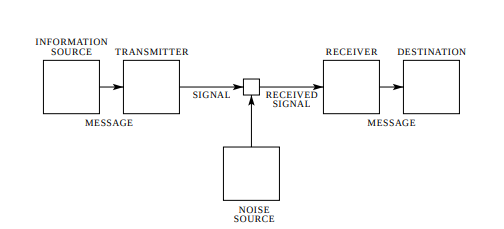
\includegraphics[width=0.65\textwidth]{comunicadorshannon.png}
  \fonte{\textcite[p. 380]{MTC}.}
\end{figure}

De acordo com  a TMC, um \textit{gerador de informação} é um objeto capaz de produzir um conjunto $X$ de $n$ eventos com probabilidade de ocorrência $P(X)$, enquanto um \textit{receptor} possui um conjunto $Y$, também com $n$ eventos, com probabilidades associadas $P(Y)$. Durante a transmissão é possível que parte da informação seja perdida, devido a ocorrência de ruídos, o que resulta diretamente na modificação dos valores de probabilidade dos elementos recebidos do conjunto $Y$. Reconhecendo portanto os elementos de $X$ e suas probabilidades associadas, espera-se que uma mensagem bem transmitida, ou seja, sem interferência de ruídos, seja aquela cujas probabilidades dos elementos do conjunto $Y$ sejam as mesmas dos conjunto de elementos de $X$. Assim, se essas probabilidades forem distintas, podemos concluir que houve perda de informação na transmissão \cite{mathematical}.

De maneira geral, a informação é quantificada de acordo com os recursos físicos necessários para que ela seja representada, ou seja, na capacidade de armazenamento, comunicação e representação de um conjunto $X$ de possíveis informações. Em um computador clássico, por exemplo, armazenamos informações através das unidades binárias chamadas \textit{bits}\footnote{Nome proposto, segundo o artigo original de Shannon por J.W. Turkey \cite{MTC}.} Dessa forma, os bits são a menor unidade de armazenamento de informação em um computador de arquitetura clássica, podendo representar o estado 1 ou o estado 0 \cite{MTC}.

A combinação desses bits faz com que uma mensagem possa ser armazenada, processada ou transmitida em um computador clássico. Nesse sentido, quão maior, ou ainda, quão mais complexa for a mensagem a se operar, mais bits serão necessários e consequentemente mais recursos físicos para a representação destes. Com a evolução dos computadores e consequentemente com a necessidade de um maior número de bits a se operar, ocorreu um processo de miniaturização do hardware, em particular, do dispositivo transistor. Com transistores cada vez menores, menos espaço físico era necessário para operar a informação e cada vez mais informação era possível de ser operada simultaneamente. Basta recordar que o tamanho de um smartphone moderno é muito menor do que a primeira unidade de computador eletrônico criado, o ENIAC que ocupava um espaço de \SI{180}{\square\meter} \cite{eniac}.

Porém, em 1965 foi estabelecido por Gordon E. Moore um limite de processamento devido ao número de transistores necessários comprimidos em um pequeno espaço, versus sua dissipação de calor, o que corrompe a informação. Esse limite recebeu o nome de ``Lei de Moore''. Nela, \textcite{moore} estima que o número de transistores de um computador dobraria a cada dois anos sem que seu valor fosse alterado. Esse limite foi brevemente superado por novas tecnologias de materiais\footnote{A empresa IBM, produziu em 2014 um nanochip de silício de 7 nm e em 2015 anunciou a produção de chips de processamento com nanotubos de carbono de tamanho 1,8nm \cite{chipibm}.}, deixando evidente, entretanto, a necessidade de expandir a capacidade de processamento dos sistemas atuais, visto que a tendência de crescimento na quantidade de informação processada é cada vez maior.

Em 1981, o físico Richard Feynman, em um de seus seminários, sugeriu que os conceitos de Mecânica Quântica fossem aplicados à computação para que a informação pudesse ser operada de maneira mais rápida e em maior quantidade \cite{TeoQuanInfoEntreCopia}.

A Mecânica Quântica é o ramo da Física que surge na virada do século XX a partir de uma série de experimentos que não puderam ser explicados classicamente. As hipoteses produzidas por nomes como Planck, Eistein, Bohr e De Broglie e posteriormente aperfeiçoadas por Schrödinger, Heisenberg e Dirac, descrevem uma nova área na Física. Para o desenvolvimento de um computador de arquitetura quântica, destacamos a importância do \textit{Princípio da Superposição de Estados}.

O Princípio da Superposição de Estados determina que um estado de um sistema físico é composto por todas as informações possíveis de serem extraídas dele em uma medição. Disso ocorre que um estado possui definição probabilística a partir de todos as possibilidades de ocupação deste. Esses estados são representados por um vetor do espaço complexo de Hilbert $H$, chamados também, usando a notação de Dirac, de \textit{kets} e representados por $\ket{\psi}$.

Nesse sentido, unindo a teoria quântica às necessidades de aumento no processamento de informação, surge uma nova área de estudo, a \textit{Computação Quântica}. Segundo \textcite{CompInfoQuantica} e \textcite{dwave}, a devida construção de um computador de arquitetura quântica foi precedida pelos eventos descritos a seguir:

\begin{description}
  \item[1985] David Deustch propõe matematicamente o primeiro computador quântico universal;
  \item[1994] Peter Shor cria o primeiro programa essencialmente quântico, ou seja, ele não poderia ser executado em um computador clássico. Este programa, conhecido como Algoritmo de Shor, reduziria o tempo de fatoração de números grandes de possíveis meses para apenas segundos caso fosse utilizado em um computador real de arquitetura quântica;
  \item[1999] O MIT apresenta o primeiro protótipo de um computador quântico real;
  \item[2007] A empresa D-Wave apresenta o primeiro computador essencialmente quântico.
\end{description}

A descrição da arquitetura de um computador quântico esbarra no mesmo princípio daquela de um computador clássico, ou seja, em sua unidade fundamental de armazenamento de informação. De maneira análoga ao computador clássico, que utiliza como unidade de informação o bit, o computador quântico utilizará o \textit{qubit} (ou q-bit, ou ainda, quantum bit).

Um qubit, ou bit quântico, pode ser produzido de maneiras distintas\footnote{Qubits podem ser fisicamente criados utilizando, por exemplo, spins de átomos presos em uma armadilha. Essa armadilha pode ser do tipo óptica ou até mesmo magnética. É possível também polarizar fótons para sua obtenção. A determinação do método é definida principalmente pelo mecanismo que melhor conseguir isolar o \textit{qubit}, já que este é facilmente influenciado pelo ambiente externo \cite{materialdidaticomecquantica}.}, porém nosso foco de estudo está nas suas propriedades. Um qubit é uma unidade com propriedades quânticas que atua sob o regime de superposição de estados. Isso significa que ele consegue armazenar simultaneamente mais de um estado de informação, diferente do bit clássico que armazena apenas um dos estados por vez. Decorre desta propriedade a maior capacidade de operar a informação em comparação aos mecanismos clássicos segundo apresentado na Tabela~\ref{tabelabit}.

\begin{table}[ht!]
  \centering
  \caption{Comparação entre a quantidade de bits clássicos e quânticos necessários para se operar uma informação.}\label{tabelabit}
  \begin{tabular}{ccc}
    \toprule
    \thead{Quantidade \\ de bytes} & \thead{Quantidade \\ de bits clássicos} & \thead{Quantidade \\ de qubits} \\
    \midrule
    1         & 8            & 3  \\
    \num{e6}  & \num{8.3e6}  & 23 \\
    \num{e12} & \num{8.8e12} & 43 \\
    \bottomrule
  \end{tabular}
  \fonte{Elaborada pelo autor.}
\end{table}

De modo a generalizar a comparação entre bits classicos e quânticos, podemos estabelecer a relação:
\begin{equation} \label{bitvsqubit}
n\, \text{qubits} = 2^{n}\,\text{bits}.
\end{equation}
Portanto, podemos concluir que menos qubits são necessários para operar a informação, em comparação ao bit clássico, o que está diretamente relacionado com a velocidade e com a capacidade de realização deste.

A descrição de um qubit consiste em uma combinação linear de dois possíveis estados quânticos $\ket{0}$ e $\ket{1}$ de modo que:
\begin{equation} \label{comblinearqubit}
 \ket{\psi} = \alpha \ket{0} + \beta \ket{1}, \quad \text{com } \alpha^{2} + \beta^{2} = 1,
\end{equation}
sendo $\alpha$ e $\beta$ as amplitudes probabilísticas dos estados quânticos $\ket{0}$ e $\ket{1}$.

É interessante observar que, apesar de qubits conseguirem armazenar mais informação devido à superposição de estados, a obtenção direta desta é impossível visto que, diferente da mecânica clássica, onde podemos observar se um bit se encontra em um estado 0 ou um estado 1, em situações quânticas a observação faz com que o sistema colapse. Portanto, o foco de aproveitamento de um qubit está em conseguir transferir a informação que ele armazena, sem que uma medida seja realizada diretamente nesta unidade quântica \cite{chuang}.

Apesar dessa aparente dificuldade em se obter a informação quântica, existem alguns mecanismos que facilitam e possibilitam sua obtenção. Segundo \textcite{materialdidaticomecquantica}, para a compreensão destes mecanismos serão necessários estabelecer alguns teoremas que regem a informação quântica.

\begin{theo}{não-clonagem}{teo1}
É impossível clonar um estado quântico, ou seja, qualquer dispositivo que receba um estado quântico como entrada, será incapaz de reproduzir como saída exatamente o mesmo estado quântico.
\end{theo}

\begin{theo}{}{teo2}
Não é possível obter um estado quântico desconhecido de um sistema único e individual realizando uma medição sobre este, independente do tipo e/ou sequência de medições que se realize.
\end{theo}

Pelos Teoremas~\ref{th:teo1} e~\ref{th:teo2} parece ser improvável a proposta de que a informação quântica se sobressaia em relação à clássica, mas é exatamente devido a eles e aos mecanismos que estes proporcionam destes que a informação quântica se torna tão promissora. Os mecanismos que estudaremos nesse trabalho são o \textit{Emaranhamento (ou Entrelaçamento) Quântico} e o \textit{Teletransporte Quântico}.

O Emaranhamento Quântico é uma consequência quântica proveniente da superposição de estados de elementos dessa natureza. Vale ressaltar que objetos e fenômenos quânticos nem sempre possuem o análogo clássico, como o caso de spins. Nesse fenômeno duas particulas interagem de modo que o estado quântico de uma delas não pode ser mais descrito sem o da outra. Isso faz com que, mesmo que as partículas estejam distantes uma da outra, elas continuam a compartilhar os estados quânticos. Isso faz com que seja possível, conhecendo algumas propriedades de uma das partículas com por exemplo a posição, seja possível determinar esta mesma característica da outra partícula. A determinação das propriedades de uma das partículas culmina na instantânea definição na segunda, pois elas compartilham o mesmo estado quântico, o que nos leva a utilização do Emaranhamento para a realização do Teletransporte Quântico \cites{materialdidaticomecquantica}{fonzar}{TeoQuanInfoEntreCopia}.

O Teletransporte Quântico consiste em uma série de operações realizadas por intermédio de um circuito de natureza quântica que pretende enviar uma mensagem de um ponto \(A\) até um ponto \(B\). Para a realização desse procedimento, dependemos essencialmente de ao menos três qubits. Para introduzir esse conceito, iremos nos apropriar de uma história hipotética a título de esclarecer a ideia principal do fenômeno. Imagine por um instante que se deseja enviar uma fotografia para alguém que não se vê há muito tempo. Existem essencialmente duas maneiras de realizar o envio: pode-se enviar a foto pelo correio e aguardar que o destinatário a receba, processo chamado de transporte de informação, ou ainda, você poderia criar um arquivo digital com informações sobre a fotografia, de maneira que aquele que recebe o arquivo, possa de alguma maneira recriar a foto; nesse segundo caso, a foto seria teletransportada \cite{materialdidaticomecquantica}.

Trazendo a situação descrita para o universo quântico, o teletransporte de estados quânticos consiste em uma série de operações que possibilitam descrever no ponto \(B\) um estado existente no ponto \(A\). A princípio, devido ao Teorema~\ref{th:teo1} da não-clonagem\footnote{A informação clássica pode ser facilmente reproduzida, basta recordar que um livro pode ser impresso com a tiragem de exemplares desejada. Já a informação quântica não é plausível de reprodução direta. Algumas provas matemáticas desta impossibilidade são apresentadas em \textcite{TeoQuanInfoEntreCopia}.}, seria impossível ``clonar'' um qubit, ou seja, teletransportar a informação de modo semelhante ao que ocorre com um canal clássico. Porém, segundo \textcite{bennet}, é possível contornar o problema utilizando um canal de informação clássico, semelhante ao apresentado por Shannon na TMC, porém utilizando como emissor-receptor um par de partículas emaranhadas quanticamente.

Na literatura encontram-se as mais diversas explicações sobre como funciona o teletransporte quântico \cites{bennet}{experimentalqt}{zeilinger}{brassard1996teleportation}{materialdidaticomecquantica} e na maioria dos casos, os leitores são introduzidos a dois personagens: Alice e Bob.

Na história, os cientistas Alice e Bob estão localizados em dois laboratórios distintos, cada um deles possui um qubit, $q_{A}$ e $q_{B}$ e estes estão emaranhados, produzindo um estado quântico emaranhado denominado de $\ket{\psi_{AB}}$. Alice precisa enviar uma mensagem urgente para Bob utilizando um outro qubit, $q_{C}$. Portanto, no início do processo de teletransporte, Alice possui dois qubits, o que ela deseja enviar e o que possui o estado quântico emaranhado com o qubit de Bob.

Alice realiza então uma série de operações entre seus qubits e, como um deles está emaranhado com o de Bob, este saberá que algo está mudando. Para continuar o processo de teletransporte, Alice faz uma medição em seus qubits, colapsando-os e envia, via um canal clássico, a informação dos qubits colapsados para Bob. Este por sua vez, por saber qual era o estado inicial de $q_{A}$ devido ao emaranhamento, conseque reconstruir a mensagem presente originalmente no qubit $q_{C}$ enviado por Alice. Portanto, a mensagem é reconstruida e não clonada, não violando o princípio da não-clonagem (Teorema~\ref{th:teo1}). A não clonagem fica explicitada no momento em que a medida é realizada em $q_{A}$ e $q_{C}$, colapsando-os, de modo que existe apenas uma cópia do estado de $q_{C}$ dado por $\ket{\psi_{C}}$.

O teletransporte quântico possui algumas questões que devem ser salientadas. A primeira delas é que, de fato, este é um método de transmissão de informação extremamente seguro, visto que, se o receptor não tiver o qubit emaranhado com o do emissor, a mensagem não poderá ser recuperada, além do fato de que a informação original é destruída na transmissão da mensagem. Disso decorre imediatamente a segunda questão. A informação pode, eventualmente, sofrer interferências de ruídos externos durante seu envio e por não possuir mais a mensagem original, pode ser perdida.

Portanto, o estudo dos possíveis ruídos que possam interferir no teletransporte, assim como na transmissão clássica, faz com que, mesmo que estes ocorram, seja possível recuperar a informação ao final do processo, corrigindo-os. Existem os mais diversos tipos de ruídos aos quais a mensagem pode ser exposta, o que torna praticamente impossível prever quais deles efetivamente ocorreram ao recuperar uma mensagem; porém, o estudo de ruídos familiares torna possível o reconhecimento destes tornando mais provável a recuperação da informação enviada \cite{fonzar}.

A construção do sistema de teletransporte quântico demanda um circuito onde operam as chamadas \textit{portas lógicas quânticas} e portanto, a realização experimental de um teletransporte quântico demanda efetivamente um computador de arquitetura quântica para que as operações ocorram sob os qubits. Apesar de já existirem computadores quânticos, ainda são necessários estudos acerca deste para que cada vez mais a qualidade dos qubits seja melhorada. Porém, devido aos recursos de simulação, podemos utilizar um computador de arquitetura clássica para simular tanto um qubit quanto os circuitos lógicos necessários para a realização do teletransporte quântico, a título do estudo, por exemplo, dos efeitos de ruídos na transmissão da informação quântica conforme propomos nesse trabalho.



\clearpage


%\begin{citacao}
 % \color{red}
%  Citação direta com mais de 3 linhas, deve ser digitada com letra em tamanho menor da que foi utilizada no texto, sem aspas, e com recuo de 4 cm da margem esquerda e espaçamento simples. Deve-se mencionar, além do sobrenome do autor e data de publicação, o(s) número(s) da página de onde retirou a citação \cite[p. 32]{Collobert2011}.
%\end{citacao}

%{\color{red}Nas citações indiretas não são colocadas ``\emph{aspas}'' e nem o número da página \cite{Collobert2011}.}

%Evitem o uso de citações diretas para o caso de definições de conceitos físicos, técnicas experimentais ou mesmo para opiniões de outros autores. Na maioria das vezes não é necessário fazer esse tipo de citações. Dê preferência para as citações indiretas. Leiam o texto referido até vocês entenderem e poderem expressar as ideias e conceitos por trás dos mesmos com as próprias palavras. Com isso vocês evitam que o texto de vocês seja composto por vários recortes de dizeres de outros autores. A citação direta é usualmente utilizada quando queremos expressar exatamente o que o autor citado escreveu.

%No caso de ser necessário fazer uma citação indireta, como uma citação de uma citação, utilizem a palavra latina ``\emph{apud}'', cujo significado é ``\emph{junto a, perto de, em}'', mas que no contexto científico e acadêmico é utilizado como sinônimo de ``\emph{citado por}''. Especificamente, quando você utilizar o apud significa que você está citando a obra de um autor que você não leu, mas que foi citada na obra de outro autor cuja obra você leu e estudou. Isso ocorre comumente quando livros muito antigos e que não estão disponíveis em formato eletrônico ou mesmo impresso são citados. Isso pode ocorrer também quando vocês não têm acesso à revista (acesso pago) em que o artigo original foi publicado. Veja o exemplo:

%De acordo com \textapud[p. 148]{Collobert2011}[p. 8]{Souza2010} a estabilidade de um foguete de garrafas PET pode ser obtida se o centro de massa do foguete estiver em torno de \SI{1.5}{\centi\meter} acima do seu centro de pressão.

%As normas exigidas neste trabalho para a citação de livros e revistas são impostas automaticamente pelo estilo de ABN{\TeX}2. Vale ressaltar que não existe o padrão mais correto para a escrita de projetos e artigos científicos, o que existe são padrões e normativas exigidos. Um dos objetivos deste trabalho é aprender a seguir um padrão.

%Apesar de toda a riqueza da língua portuguesa e inglesa para a escrita expositiva, o estilo da escrita científica é puramente técnico e conciso. Esta deve ser o mais claro possível, evitem utilizar uma linguagem barroca, rebuscada, transforme o texto de vocês em algo poderoso e convincente com simples e poucas palavras, evitem redundâncias. Isso é válido para projetos e artigos científicos, dissertações de mestrado, teses de doutorado e relatórios de prática. {\color{red}Com relação ao tempo verbal para a escrita do projeto, este deve estar no futuro, pois o projeto consiste de uma proposta que será executada no decorrer da graduação de vocês e finalizada, provavelmente, quando vocês cursarem a disciplina de TCC 2.} 

%{\color{red}Mesmo que vocês escrevessem o projeto sozinhos, um único autor, utilizem o que chamamos de ``\emph{eu formal}'', que consiste em se referir às atividades de pesquisa na primeira pessoa do plural.} É como se vocês estivessem convidando o leitor para participar do projeto, por exemplo, ``\emph{Neste projeto desenvolveremos\ldots executaremos\ldots pesquisaremos sobre\ldots etc.}'' Em relatórios de prática é usual utilizarmos o tempo verbal na terceira pessoa, como ``\emph{foi feito\ldots foi analisado\ldots foi executado\ldots foi estabelecido\ldots etc.}'' Neste caso não existe autoria sobre o que foi desenvolvido, pois trata-se de uma reprodução, geralmente orientada através de um roteiro. Em um projeto ou artigo científico é importante exaltar a autoria do trabalho de vocês. Terceira pessoa será utilizada para os trabalhos de outros autores, pois vocês precisarão citar o que já foi feito por outros pesquisadores no tema escolhido. Quando vocês escrevem nós, fica claro o que foi realmente feito por vocês. Esta é uma tendência que já está sendo sugerida em várias revistas e jornais do mundo todo.

%\noindent
%\textbf{\color{red}IMPORTANTÍSSIMO:} Quando vocês forem utilizar informações de outras fontes, como definições ou técnicas experimentais específicas evitem se remeter ao texto original diretamente. Ou seja, não copiem na íntegra as frases de outros autores. Isso é plágio! No Brasil é considerado como crime pelo código penal (Art. 184) e em outros países trata-se de uma prática antiética e extremamente desrespeitosa. Para vocês se tornarem autores profissionais, competentes e respeitados leiam o artigo, revista ou livro até entenderem a ideia que vocês pretendem abordar na proposta, descrevendo a mesma com as próprias palavras. A ideia pode ser a mesma, mas cada um tem sua maneira de se expressar. É esta a razão de termos diversos autores de livros didáticos falando sobre os mesmos tópicos de um determinado assunto. Se vocês não forem capazes disso é porque o assunto ainda não foi entendido, o que significa que mais estudos precisam ser conduzidos. Em ciência procedemos dessa forma, o entendimento sobre qualquer assunto é efetivado quando vocês são capazes de processar a informação de modo a poder expressar os conceitos com as próprias palavras.

%%%
%%% OBJETIVOS
%%%
\section{Objetivo(s) da Proposta}\label{sec:objs}

O objetivo principal deste trabalho consiste em realizar um estudo acerca dos efeitos de possíveis ruídos no fenômeno de teletransporte quântico, utilizando uma simulação de circuitos quânticos em um computador de arquitetura clássica. Para atingir tal proposta, pretende-se:
\begin{enumerate}
\item Definir o conceito de Teletransporte Quântico;
\item Delinear as situações onde o fenômeno é utilizado;
\item Elencar os tipos de ruídos que podem interferir na transmissão de informação durante o fenômeno;
\item Construir a simulação de comportamento de um \textit{qubit};
\item Estruturar as portas lógicas quânticas a serem simuladas para o presente estudo;
\item Estabelecer uma sequência de testes com os algoritmos de ruído;
\item Comparar os resultados obtidos na simulação desenvolvida com os resultados provenientes de simuladores em computadores de arquitetura quântica como o IBM Quantum e o Azure Quantum.
\end{enumerate} 

%\subsection{Nome do tópico 1}\label{obj1}

%Descreva a importância do tópico 1 para a execução do seu projeto de pesquisa \cites{vene2008}{Collobert2011}{braess2007}.


%\subsection{Nome do tópico 2}\label{obj2}

%Descreva a importância do tópico 2 para a execução do seu projeto de pesquisa e assim por diante.

%Caso vocês e os respectivos orientadores prefiram iniciar uma nova seção para isso, como por exemplo: \emph{Fundamentação Teórica} ou algum título específico sobre o que será abordado no projeto não tem problema. O importante é que o projeto fique bem organizado e o assessor capte com facilidade a proposta e os principais conceitos a serem abordados no trabalho. O uso de subseções na seção de objetivos é apenas sugestivo.

%\subsection{Nome do tópico 3}\label{obj3}

%E por ai vai\ldots

%%%
%%% METODOLOGIA
%%%
\section{Metodologia}

%Descreva sua proposta metodológica de maneira detalhada seja ela experimental, através de técnicas específicas, ou teórica, desenvolvida matematicamente através de modelos analíticos ou simulações computacionais. Quais processos ou materiais vocês pretendem utilizar? Que tipos de equipamentos serão necessários?

%\noindent
%\textbf{\color{red}IMPORTANTE:} Se for necessário na apresentação de quaisquer tópicos listados acima o uso de figuras para melhorar o entendimento da mesma, siga o exemplo da Figura~\ref{fig1} abaixo. Lembrando que não existe um padrão geral para isso. Seguiremos as normas da ABNT para o projeto. Siga a formatação dos exemplos abaixo.

%{\color{red}Figuras ilustrativas podem ser coloridas ou em preto e branco. As ilustrações devem ser esclarecedoras, nítidas e com boa resolução (300 dpi ou mais). Se houver palavras ou números na figura faça com que o tamanho da fonte seja o mais próximo possível do tamanho da fonte do texto. Todas as Figuras devem ser numeradas e citadas no texto. ESTAS DEVEM SER ESCLARECEDORAS, NÍTIDAS E COM BOA RESOLUÇÃO.}

%\begin{figure}[ht!]
%  \centering
%  \caption{Esquema ilustrativo mostrando o aparato utilizado para colocar a vela em movimento retilíneo acelerado através da queda de uma massa de \(m = \SI{50}{\gram}\). O sistema é composto por (1) mesa, (2) plataforma de madeira, (3) carrinho de plástico, (4) base de madeira, (5) vela, (6) tubo de vidro aberto, (7) barbante, (8) roldana de varal de roupas, (9) cilindro de aço e (10) régua para liberar o sistema.}\label{fig1}
%  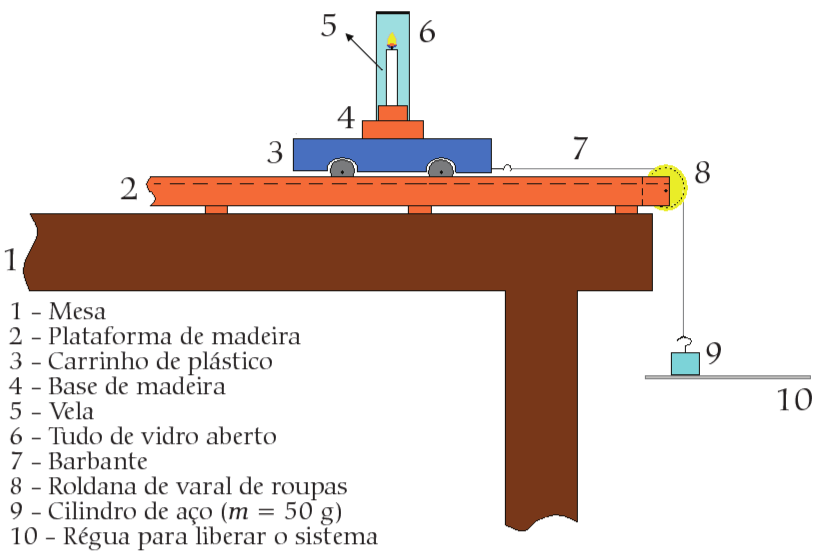
\includegraphics[width=0.65\textwidth]{fig1.png}
%  \fonte{\textcite[p. 37]{Souza2010}.}
%\end{figure}

%Outro exemplo é a ilustração de um pêndulo simples, mostrado na Figura~\ref{fig2} {\color{red}(citar as figuras no texto desta forma)}, em que uma massa \(m\) presa a um fio de comprimento \(l\) oscila em torno de seu ponto de equilíbrio com ângulo \(\theta\) sob a ação da força da gravidade. Note que a legenda da Figura~\ref{fig2} contém basicamente as mesmas informações descritas no parágrafo acima, reforçando a ideia de que uma Figura deve ser independente do texto.

%\begin{figure}[ht!]
 % \centering
%  \caption{Pêndulo simples, mostrando uma massa \(m\) presa a um fio de comprimento \(l\) oscilando com ângulo \(\theta\) em torno do ponto de equilíbrio.}\label{fig2}
%  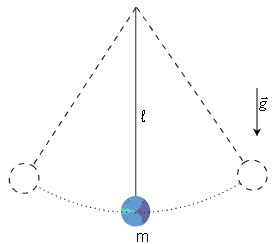
\includegraphics[width=0.4\textwidth]{pendulo.png}
%  \fonte{Elaborada pelo autor.}
%\end{figure}

%\textcolor{red}{\textbf{Observação:} As figuras, tabelas, ilustrações, etc., devem estar juntas com suas legendas e suas fontes na mesma página. A figura não pode ficar em uma página e sua legenda ou fonte em outra.}

%Se for necessário incluir alguma foto tirada por vocês mesmos ou uma foto retirada da internet siga o exemplo da Figura~\ref{fig3}.

%Quando for necessário discutir ou apresentar equações em qualquer seção do projeto, estas devem ser numeradas e citadas no texto de acordo com o número. Veja o exemplo abaixo:

%O período de oscilação \(T\) de um pêndulo simples pode ser calculado através da seguinte expressão:

%\begin{equation}\label{periodo}
%    T = 2 \pi \sqrt{\dfrac{l}{g}},
%\end{equation}
%sendo $l$ o comprimento do fio que sustenta a massa $m$ do pêndulo e $g$ a aceleração da gravidade.

%\noindent
%{\textbf{\color{red}IMPORTANTE:} Todos os parâmetros das equações devem ser explicados no texto, como neste exemplo.}

%Se o comprimento $l$ do fio for dado podemos utilizar a Equação~\eqref{periodo} ({\color{red}citar as equações no texto desta forma}) para determinar a aceleração da gravidade através da medida do período de oscilação do pêndulo.

%\begin{figure}[ht!]
%  \centering
%  \caption{Tubo de chama de onda estacionária.}\label{fig3}
%  \vspace{1mm}
%  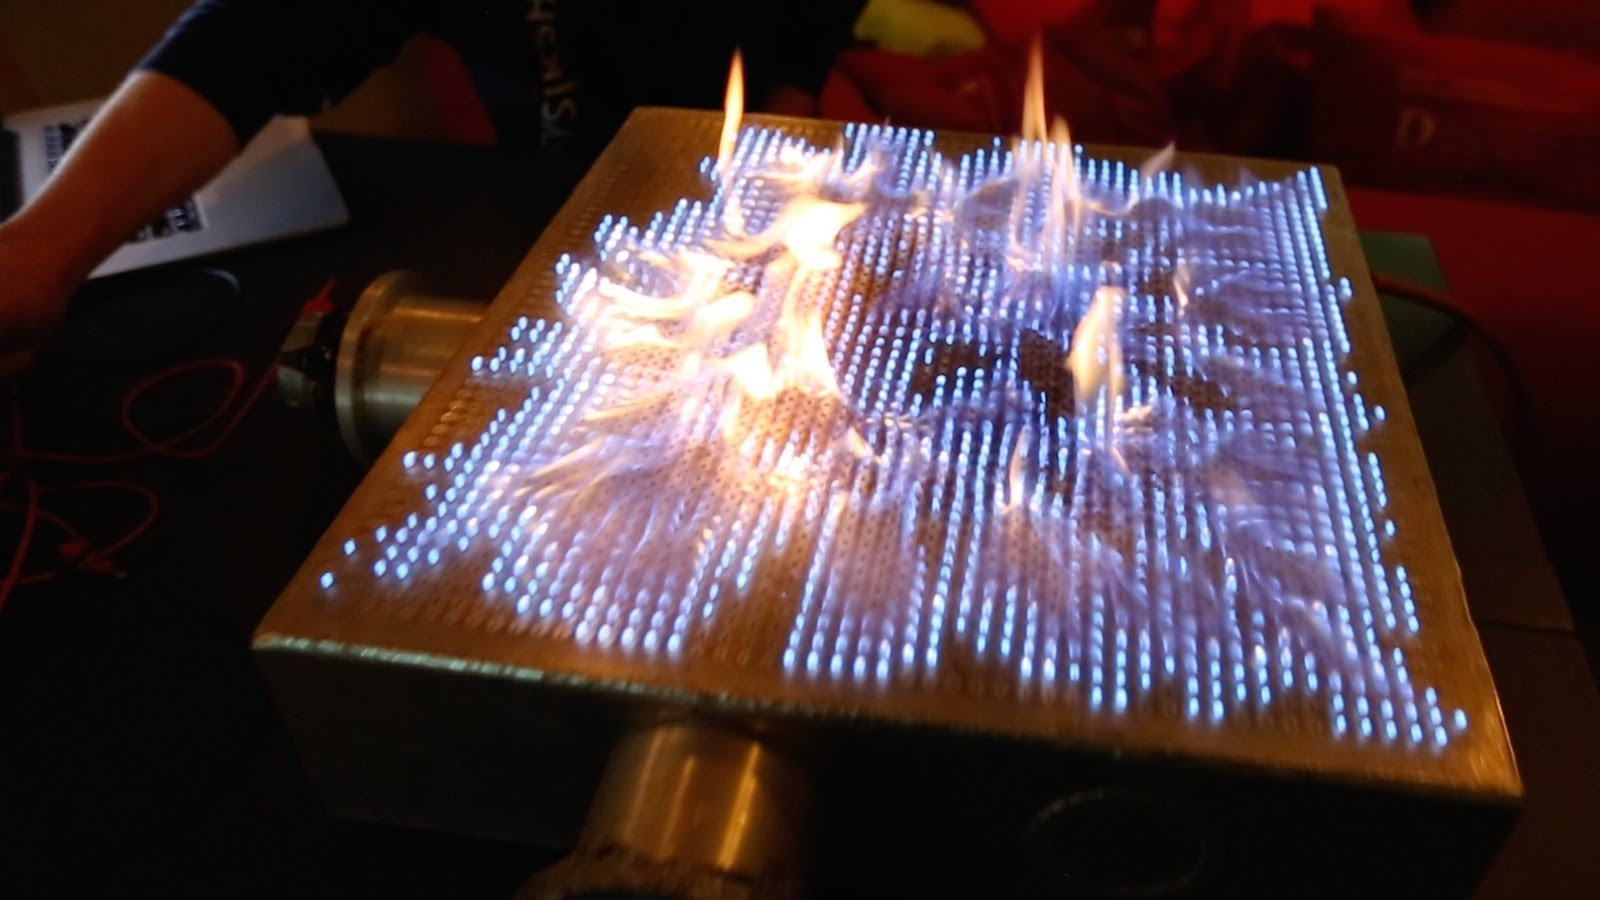
\includegraphics[width=0.6\textwidth]{Chamas.jpg}
%  \fonte{JUNIOR, G. \underline{Usando Física para criar um incrível experimento com Fogo e Música.} Disponível em: \url{http://marteeparaosfracos.blogspot.com/2014/04/usando-fisica-para-criar-um-incrivel.html}. Acesso em: 16 nov. 2018.}
%\end{figure}

%%%
%%% CRONOGRAMA
%%%
\section{Cronograma de Atividades}

%Este tópico é importante para vocês mostrarem aos assessores que avaliarão o projeto, ou no caso para o professor-orientador da disciplina de TCC 1, como vocês pretendem executar a proposta diante do prazo disponível ou determinado. Listem as tarefas que serão executadas em determinado período como pesquisa bibliográfica, busca de materiais para realização do experimento, montagem ou construção do experimento, análise dos resultados obtidos, etc. Esta pode ser feita através de uma tabela. Se caso for necessário incluir outras tabelas na proposta de pesquisa siga o modelo da Tabela~\ref{tabela1} abaixo.

%\begin{table}[ht!]
%  \centering
%  \caption{Cronograma tentativo de atividades.}\label{tabela1}
%  \begin{tabular}{cc}
%    \toprule
%    \textbf{\emph{Período}} & \textbf{\emph{Atividades}}\\
%    \midrule
%    3 primeiros meses      & Aquisição de materiais para a realização do experimento;        \\
%    2º semestre de 2021    & Montagem e testes do experimento;                               %\\
%    E assim por diante ... & O período pode ser especificado em semanas, meses ou semestres. \\
%    \bottomrule
%  \end{tabular}
%  \fonte{Elaborada pelo autor.}
%\end{table}

%É importante que o cronograma tentativo apresente de maneira clara o início das atividades, sua execução e a finalização das mesmas, com uma previsão de discussão dos resultados para a escrita da monografia final e a defesa do TCC.

%\begin{table}[ht!]
%  \begin{center}
%    \caption{Cronograma de desenvolvimento do projeto. Cada linha corresponde
%      a um objetivo específico da Seção~\ref{sec:objs}. Cada coluna
%      corresponde a um mês.}\label{tab:cronog}
%    \begin{ganttchart}[hgrid,
%                      vgrid,
%                      bar/.append style={fill=blue!10,draw=blue},
%                      bar top shift=0.1,
%                     bar height=0.8,
%                      x unit=20mm,
%                      y unit chart=6mm]{1}{6}
%      \gantttitle{Meses}{6} \\
%      \gantttitlelist{1,...,6}{1} \\
%      \ganttbar{Seção~\ref{obj1}}{1}{2} \\
%      \ganttbar{Seção~\ref{obj2}}{2}{3} \ganttbar{}{5}{6} \\
%      \ganttbar{Seção~\ref{obj3}}{4}{6} \\
%    \end{ganttchart}
%    \fonte{Elaborada pelo autor.}
%  \end{center}
%\end{table}

% Imprime a bibliografia
\clearpage
\printbibliography[heading=subbibliography]

\end{document}

%%% end of skeleton_tcc_proj.tex
